% ============================================================
% FOR OVERLEAF: Uncomment the line below and comment out the
% \documentclass{article} line. The ceurart class is available
% on Overleaf via the template gallery.
% ============================================================
% \documentclass[ceurws-v2022]{ceurart}

% For local compilation without ceurart:
\documentclass[11pt,a4paper]{article}

% Packages
\usepackage[margin=2.5cm]{geometry}
\usepackage{graphicx}
\usepackage{booktabs}
\usepackage{amsmath}
\usepackage{amssymb}
\usepackage{tikz}
\usetikzlibrary{shapes.geometric, arrows.meta, positioning, fit, calc, backgrounds}
\usepackage{pgfplots}
\pgfplotsset{compat=1.18}
\usepackage{xcolor}
\usepackage{hyperref}
\usepackage{subcaption}
\usepackage{multirow}
\usepackage{array}
\usepackage{natbib}
\bibliographystyle{unsrtnat}

% CEUR-WS compatible front matter (for local compilation)
\newcommand{\copyrightyear}[1]{}
\newcommand{\copyrightclause}[1]{}
\newcommand{\conference}[1]{}
\newcommand{\tnotemark}[1]{}
\newcommand{\tnotetext}[2]{}
\newcommand{\cormark}[1]{}
\newcommand{\fnmark}[1]{}
\newcommand{\fntext}[2]{}
\newcommand{\cortext}[2]{}
\newcommand{\sep}{, }

% Colors
\definecolor{deepseekblue}{RGB}{26,115,232}
\definecolor{glmgreen}{RGB}{52,168,83}
\definecolor{kimired}{RGB}{234,51,53}
\definecolor{conforange}{RGB}{251,188,4}
\definecolor{statpurple}{RGB}{147,52,230}
\definecolor{origgray}{RGB}{95,99,104}
\definecolor{randorange}{RGB}{255,109,1}
\definecolor{consensusgreen}{RGB}{27,94,32}
\definecolor{lightblue}{RGB}{232,240,254}
\definecolor{lightgreen}{RGB}{230,244,234}
\definecolor{lightred}{RGB}{252,232,230}
\definecolor{lightyellow}{RGB}{254,249,230}
\definecolor{lightpurple}{RGB}{243,232,253}
\definecolor{darkgreen}{RGB}{27,94,32}

% Conference info
\copyrightyear{2026}
\copyrightclause{Copyright for this paper by its authors.
  Use permitted under Creative Commons License Attribution 4.0
  International (CC BY 4.0).}

\conference{ASPAI 2026: 2nd Asia-Pacific Symposium on Process and Artificial Intelligence,
  August 25--26, 2026, Asia-Pacific region}

\title{Multi-LLM Consensus for Semantic-Preserving Event Log Augmentation in Predictive Process Monitoring}

% Anonymized for double-blind review
\author{Ifrina Nuritha, Vandha Pradwiyasma Widartha, Chang-Soo Kim\\ \textit{Department of Information system, Universitas of Jember} \\ \textit{Department of Information System, Pukyong National University }}
\date{}

\begin{document}

\maketitle

\begin{abstract}
Predictive process monitoring (PPM) suffers from data scarcity in real-world event logs, which are often small, exhibit low variability, and contain class-imbalanced outcomes. While data augmentation can address these limitations, existing methods either violate process semantics---producing invalid traces such as ``Deliver before Ship''---or rely on statistical patterns derived solely from the original log, limiting their ability to generate novel yet valid behavioral variants. We propose a multi-LLM consensus framework that leverages multiple large language models with complementary capabilities to generate and verify augmented process traces. A reasoning-oriented model generates candidate traces conditioned on process model constraints, while a structured-output model and a long-context model independently verify structural validity and temporal consistency, respectively. Traces are accepted only when at least two of three verifiers agree (2-of-3 consensus), and programmatic conformance checking against a discovered Petri net serves as an additional verification layer. Experiments on the Sepsis event log demonstrate that multi-LLM consensus filtering yields higher semantic validity (conformance fitness 0.85) than statistical augmentation baselines (best 0.81) and unfiltered LLM generation (0.68), while improving next-activity prediction accuracy by 4.6 percentage points over unaugmented data.
\end{abstract}

\begin{keywords}
Process Intelligence, Event Log Augmentation, Large Language Models, Multi-Model Consensus, Predictive Process Monitoring, Conformance Checking
\end{keywords}

%% ============================================================
\section{Introduction}
%% ============================================================

Predictive process monitoring (PPM) applies machine learning to event logs to predict the future state of running process instances---typically next-activity, remaining-time, or outcome predictions~\cite{teinemaa2019outcome}. A fundamental challenge in PPM is \emph{data scarcity}: real-world event logs are often small, contain few distinct trace variants relative to total cases, and exhibit severe class imbalance in outcomes~\cite{vanstraten2025siamsa}.

Data augmentation offers a natural remedy. However, event log augmentation is fundamentally different from augmentation in computer vision or natural language processing. Event traces are sequentially dependent: activity $B$ follows activity $A$ because of a causal dependency, not random chance. Standard augmentation techniques such as SMOTE assume sample independence, an assumption violated by sequential process data~\cite{padella2025comparison}. Random insertion, deletion, or replacement of activities within traces frequently produces semantically invalid sequences---for example, delivering an order before it has been shipped~\cite{vanstraten2025siamsa}.

Recent work has begun addressing this challenge. SiamSA-PPM~\cite{vanstraten2025siamsa} proposes statistically grounded augmentation operators that preserve control-flow semantics by operating only on patterns observed in the training log. Padella et al.~\cite{padella2025comparison} provide a comprehensive benchmark comparing seven augmentation techniques, finding that process-specific methods significantly outperform traditional approaches. However, these methods are limited to recombining existing patterns and cannot generate genuinely novel yet valid behavioral variants.

Concurrently, large language models (LLMs) have shown promise for process mining tasks~\cite{berti2024pmllm,rebmann2024evaluating}, but they suffer from hallucination: generating traces that appear plausible but violate process constraints~\cite{rebmann2024evaluating}. No existing work combines LLM generative capabilities with systematic verification to produce semantically valid augmented traces.

We propose a \textbf{multi-LLM consensus framework} for semantic-preserving event log augmentation. Our approach leverages three LLMs with complementary capabilities: (1) a reasoning-oriented model (DeepSeek-R1) generates candidate traces conditioned on process model context, (2) a structured-output model (GLM-4) verifies structural conformance against the discovered directly-follows graph, and (3) a long-context model (Kimi-K2) verifies temporal ordering consistency across full trace sequences. Candidate traces are accepted only when at least two of three verifiers agree, with programmatic conformance checking against a discovered Petri net as an additional safeguard.

Our contributions are:
\begin{enumerate}
    \item The first multi-LLM consensus framework for semantic-preserving event log augmentation in process mining.
    \item A 2-of-3 voting mechanism combining LLM-based verification with programmatic conformance checking.
    \item Empirical evaluation on a public event log comparing multi-LLM augmentation against statistical baselines on semantic validity and downstream prediction accuracy.
\end{enumerate}


%% ============================================================
\section{Related Work}
%% ============================================================

\paragraph{Event Log Augmentation.}
K\"{a}ppel et al.~\cite{kappel2023modelagnostic} proposed model-agnostic random transformations (insertion, deletion, replacement) for event logs, demonstrating improved next-activity prediction. Van Straten et al.~\cite{vanstraten2025siamsa} identified that random transformations risk violating process semantics and proposed SiamSA-PPM, which applies statistically grounded operators leveraging control-flow patterns. Padella et al.~\cite{padella2025comparison} benchmarked seven augmentation techniques and found that process-specific methods significantly outperform traditional approaches, with stochastic transition systems combined with queue modeling yielding the highest quality. Wangelik et al.~\cite{wangelik2025differential} explored generative models for privacy-preserving trace generation but noted limitations with rare variants.

\paragraph{LLMs for Process Mining.}
Berti et al.~\cite{berti2024pmllm} introduced the PM-LLM-Benchmark for evaluating LLMs on process mining tasks, finding that most LLMs perform some tasks satisfactorily but struggle with challenging tasks out-of-the-box. Rebmann et al.~\cite{rebmann2024evaluating} showed that LLMs fail on semantics-aware PM tasks without fine-tuning. Pyrih et al.~\cite{pyrih2025instruction} demonstrated that instruction-tuned LLMs show significant improvement on process discovery and prediction but remain unreliable on anomaly detection. Fionda et al.~\cite{fionda2025declarative} revealed substantial variability in LLM performance on declarative process mining, highlighting the need for robust output assessment.

\paragraph{Multi-Model Consensus.}
The concept of multi-model agreement as a trust signal draws from the ``model consortium'' approach~\cite{karpathy2024consortium}, where multiple independent models vote on outputs and agreement increases confidence. In process mining, no prior work applies multi-model consensus for augmentation or verification, though van der Aalst~\cite{vanderaalst2025noai} has argued that Process Intelligence should serve as a grounding layer for AI, providing the ``reality check'' that individual LLMs lack.


%% ============================================================
\section{Methodology}
%% ============================================================

\subsection{Problem Definition}

Given an event log $L = \{t_1, t_2, \ldots, t_n\}$ where each trace $t_i = \langle a_1, a_2, \ldots, a_m \rangle$ is a sequence of activities, and a discovered process model $M$ (Petri net or DFG), the augmentation problem is to generate a set of synthetic traces $S = \{s_1, s_2, \ldots, s_k\}$ such that: (1) each $s_j$ is semantically valid with respect to $M$, (2) $S$ increases trace variability beyond $L$, and (3) training on $L \cup S$ improves downstream PPM performance compared to training on $L$ alone.

\subsection{Multi-LLM Consensus Framework}

Figure~\ref{fig:architecture} presents the overall architecture of our proposed framework, which consists of four stages: \emph{context extraction}, \emph{trace generation}, \emph{multi-model verification}, and \emph{consensus filtering}.

\begin{figure*}[t]
\centering
\resizebox{\textwidth}{!}{%
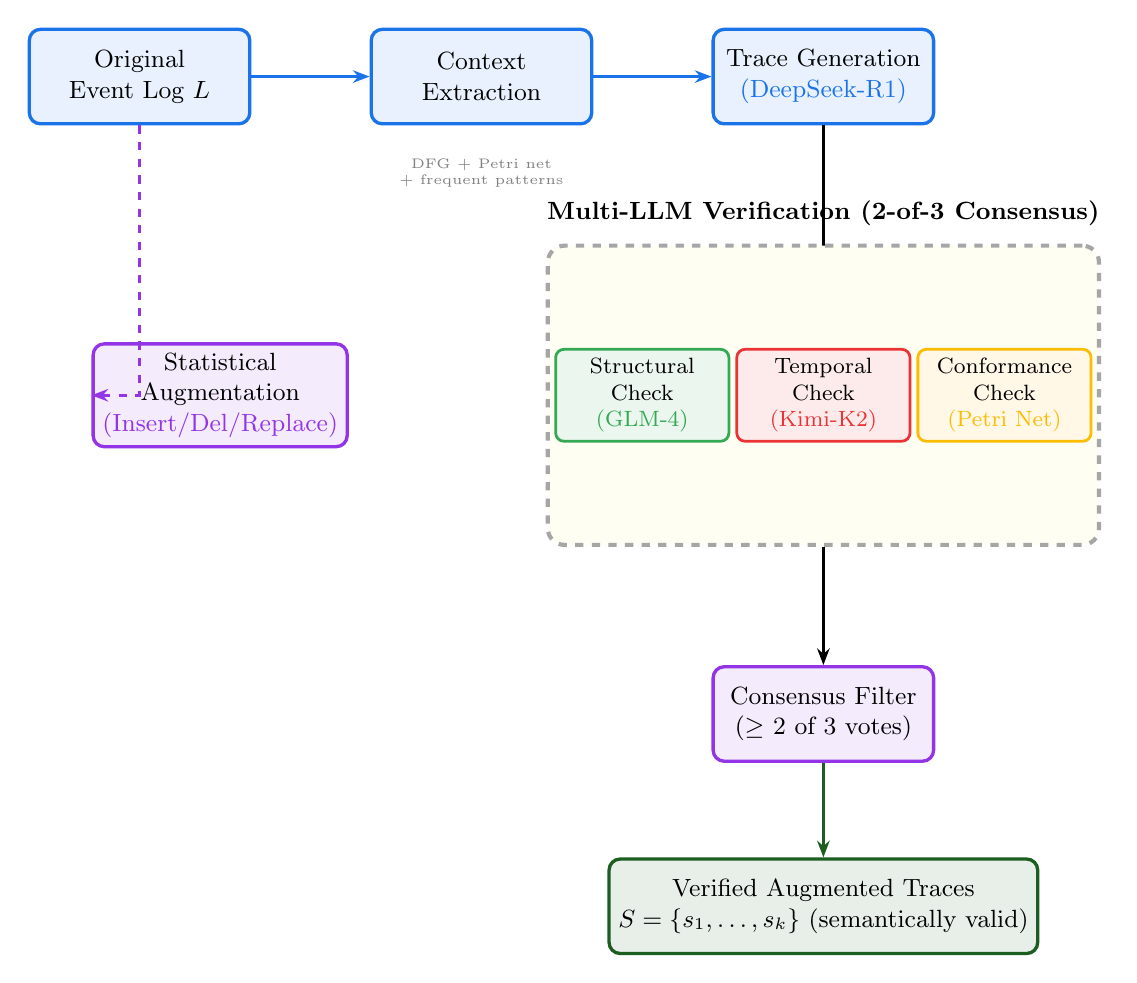
\begin{tikzpicture}[
    node distance=1.2cm and 1.5cm,
    box/.style={rectangle, rounded corners=4pt, draw=#1, fill=#1!10, line width=1.2pt,
        minimum width=2.8cm, minimum height=1.2cm, align=center, font=\small},
    smallbox/.style={rectangle, rounded corners=3pt, draw=#1, fill=#1!10, line width=1pt,
        minimum width=2.2cm, minimum height=1cm, align=center, font=\footnotesize},
    bigbox/.style={rectangle, rounded corners=6pt, draw=gray!70, fill=yellow!5, line width=1.5pt,
        dashed, minimum width=7cm, minimum height=3.8cm},
    arr/.style={-{Stealth[length=6pt]}, line width=1.2pt, color=#1},
    label/.style={font=\footnotesize\itshape, text=#1},
]

% Row 1: Input pipeline
\node[box=deepseekblue] (log) {Original\\Event Log $L$};
\node[box=deepseekblue, right=1.5cm of log] (ctx) {Context\\Extraction};
\node[box=deepseekblue, right=1.5cm of ctx] (gen) {Trace Generation\\{\color{deepseekblue}(DeepSeek-R1)}};

\draw[arr=deepseekblue] (log) -- (ctx);
\draw[arr=deepseekblue] (ctx) -- (gen);

% Arrow down to verification
\node[below=1.8cm of gen] (verstart) {};
\draw[arr=black] (gen) -- (verstart);

% Verification box
\node[bigbox, below=1.5cm of gen] (verifybox) {};
\node[above=0.1cm of verifybox.north, font=\small\bfseries] {Multi-LLM Verification (2-of-3 Consensus)};

\node[smallbox=glmgreen] (v1) at ([xshift=-2.3cm]verifybox.center) {Structural\\Check\\{\color{glmgreen}(GLM-4)}};
\node[smallbox=kimired] (v2) at (verifybox.center) {Temporal\\Check\\{\color{kimired}(Kimi-K2)}};
\node[smallbox=conforange] (v3) at ([xshift=2.3cm]verifybox.center) {Conformance\\Check\\{\color{conforange}(Petri Net)}};

% Arrow down to consensus filter
\node[box=statpurple, below=1.5cm of verifybox] (filter) {Consensus Filter\\($\geq$ 2 of 3 votes)};

\draw[arr=black] (verifybox.south) -- (filter);

% Arrow down to output
\node[box=darkgreen, below=1.2cm of filter] (output) {Verified Augmented Traces\\$S = \{s_1, \ldots, s_k\}$ (semantically valid)};

\draw[arr=darkgreen] (filter) -- (output);

% Side: Statistical augmentation
\node[box=statpurple, left=2.5cm of verifybox] (stat) {Statistical\\Augmentation\\{\color{statpurple}(Insert/Del/Replace)}};

\draw[arr=statpurple, dashed] (log.south) |- (stat.west);

% Context extraction details (below the boxes)
\node[below=0.3cm of ctx, font=\tiny, align=center, text=gray] {DFG + Petri net\\+ frequent patterns};

\end{tikzpicture}
}%
\caption{Architecture of the Multi-LLM Consensus Framework for Event Log Augmentation. The original event log is processed through context extraction, LLM-based trace generation, and multi-model verification before consensus filtering. The statistical augmentation path (left) serves as a baseline.}
\label{fig:architecture}
\end{figure*}

\textbf{Stage 1: Process Model Context Extraction.} From the training log, we extract: (i) the activity alphabet, (ii) directly-follows relations with frequency counts, (iii) start and end activities, and (iv) the top-$k$ frequent trace variants. This context $C$ is provided to all LLMs as structured input.

\textbf{Stage 2: Trace Generation.} A reasoning-oriented LLM (DeepSeek-R1) generates $N$ candidate traces conditioned on $C$. The prompt specifies that traces must: start with a valid start activity, end with a valid end activity, use only activities from the alphabet, and follow only valid directly-follows relations. Output is requested as a JSON list of activity sequences.

\textbf{Stage 3: Multi-Model Verification.} Each candidate trace is independently evaluated by three verification mechanisms:

\begin{itemize}
    \item \emph{Structural verification} (GLM-4): Checks that every adjacent activity pair in the trace exists in the discovered DFG. Low temperature (0.1) ensures deterministic evaluation.
    \item \emph{Temporal verification} (Kimi-K2): Checks that the overall temporal ordering is consistent---no impossible backward transitions, reasonable trace length, and no forbidden activity repetitions. Kimi's long-context window enables processing full trace sequences.
    \item \emph{Conformance checking} (programmatic): Token-based replay alignment against the discovered Petri net, requiring fitness $\geq 0.9$.
\end{itemize}

\textbf{Stage 4: Consensus Filtering.} A trace is accepted if at least 2 of 3 verifiers agree it is valid. This 2-of-3 mechanism mitigates individual verifier failures: a structurally valid but temporally inconsistent trace is rejected if both the temporal verifier and conformance checker disagree with the structural verifier.

\subsection{Statistical Augmentation Baselines}

We reimplement three statistically grounded augmentation operators from SiamSA-PPM~\cite{vanstraten2025siamsa}:

\begin{itemize}
    \item \emph{Statistical Insertion}: If trace contains frequent pair $(B, C)$ and intermediate $\pi$ where $(B, \pi, C)$ is also frequent, insert $\pi$ between $B$ and $C$.
    \item \emph{Statistical Deletion}: If trace contains $(B, \pi, C)$ where $\pi$ is a frequent intermediate, remove $\pi$ to obtain $(B, C)$.
    \item \emph{Statistical Replacement}: If trace contains $(D, \rho_i, E)$, replace $\rho_i$ with alternative $\rho_j$ from the same XOR-replacement set $\mathcal{R}(D, E)$.
\end{itemize}

All operators are parameterized by frequency thresholds ($\alpha, \beta, \gamma, \delta$) and maximum intermediate length $\lambda_{\max}$, ensuring only patterns observed in the training log are used.

\subsection{Evaluation Metrics}

We evaluate augmentation quality along three dimensions:

\textbf{Semantic Validity.} (1) \emph{Conformance fitness}: average trace fitness from token-based replay alignment against the reference Petri net. (2) \emph{Transition validity rate}: percentage of directly-follows relations in augmented traces that exist in the reference DFG. (3) \emph{Activity coverage}: percentage of reference activities present in augmented traces.

\textbf{Augmentation Diversity.} (1) \emph{Trace entropy}: Shannon entropy over trace variant distribution. (2) \emph{Prefix entropy}: entropy over prefix distributions. Higher values indicate greater diversity.

\textbf{Downstream Prediction.} (1) \emph{Next-activity accuracy} on a held-out test set. (2) \emph{Outcome prediction F1-score} for binary classification tasks.


%% ============================================================
\section{Experimental Setup}
%% ============================================================

\subsection{Datasets}

We use the Sepsis event log~\cite{4tu_sepsis} from the 4TU Research Data repository, a small (1,050 cases, 16 activities, $\sim$830 variants) high-variability healthcare dataset where augmentation should have the largest impact. Figure~\ref{fig:dataset} illustrates the dataset characteristics and the augmentation challenge.

\begin{figure*}[t]
\centering
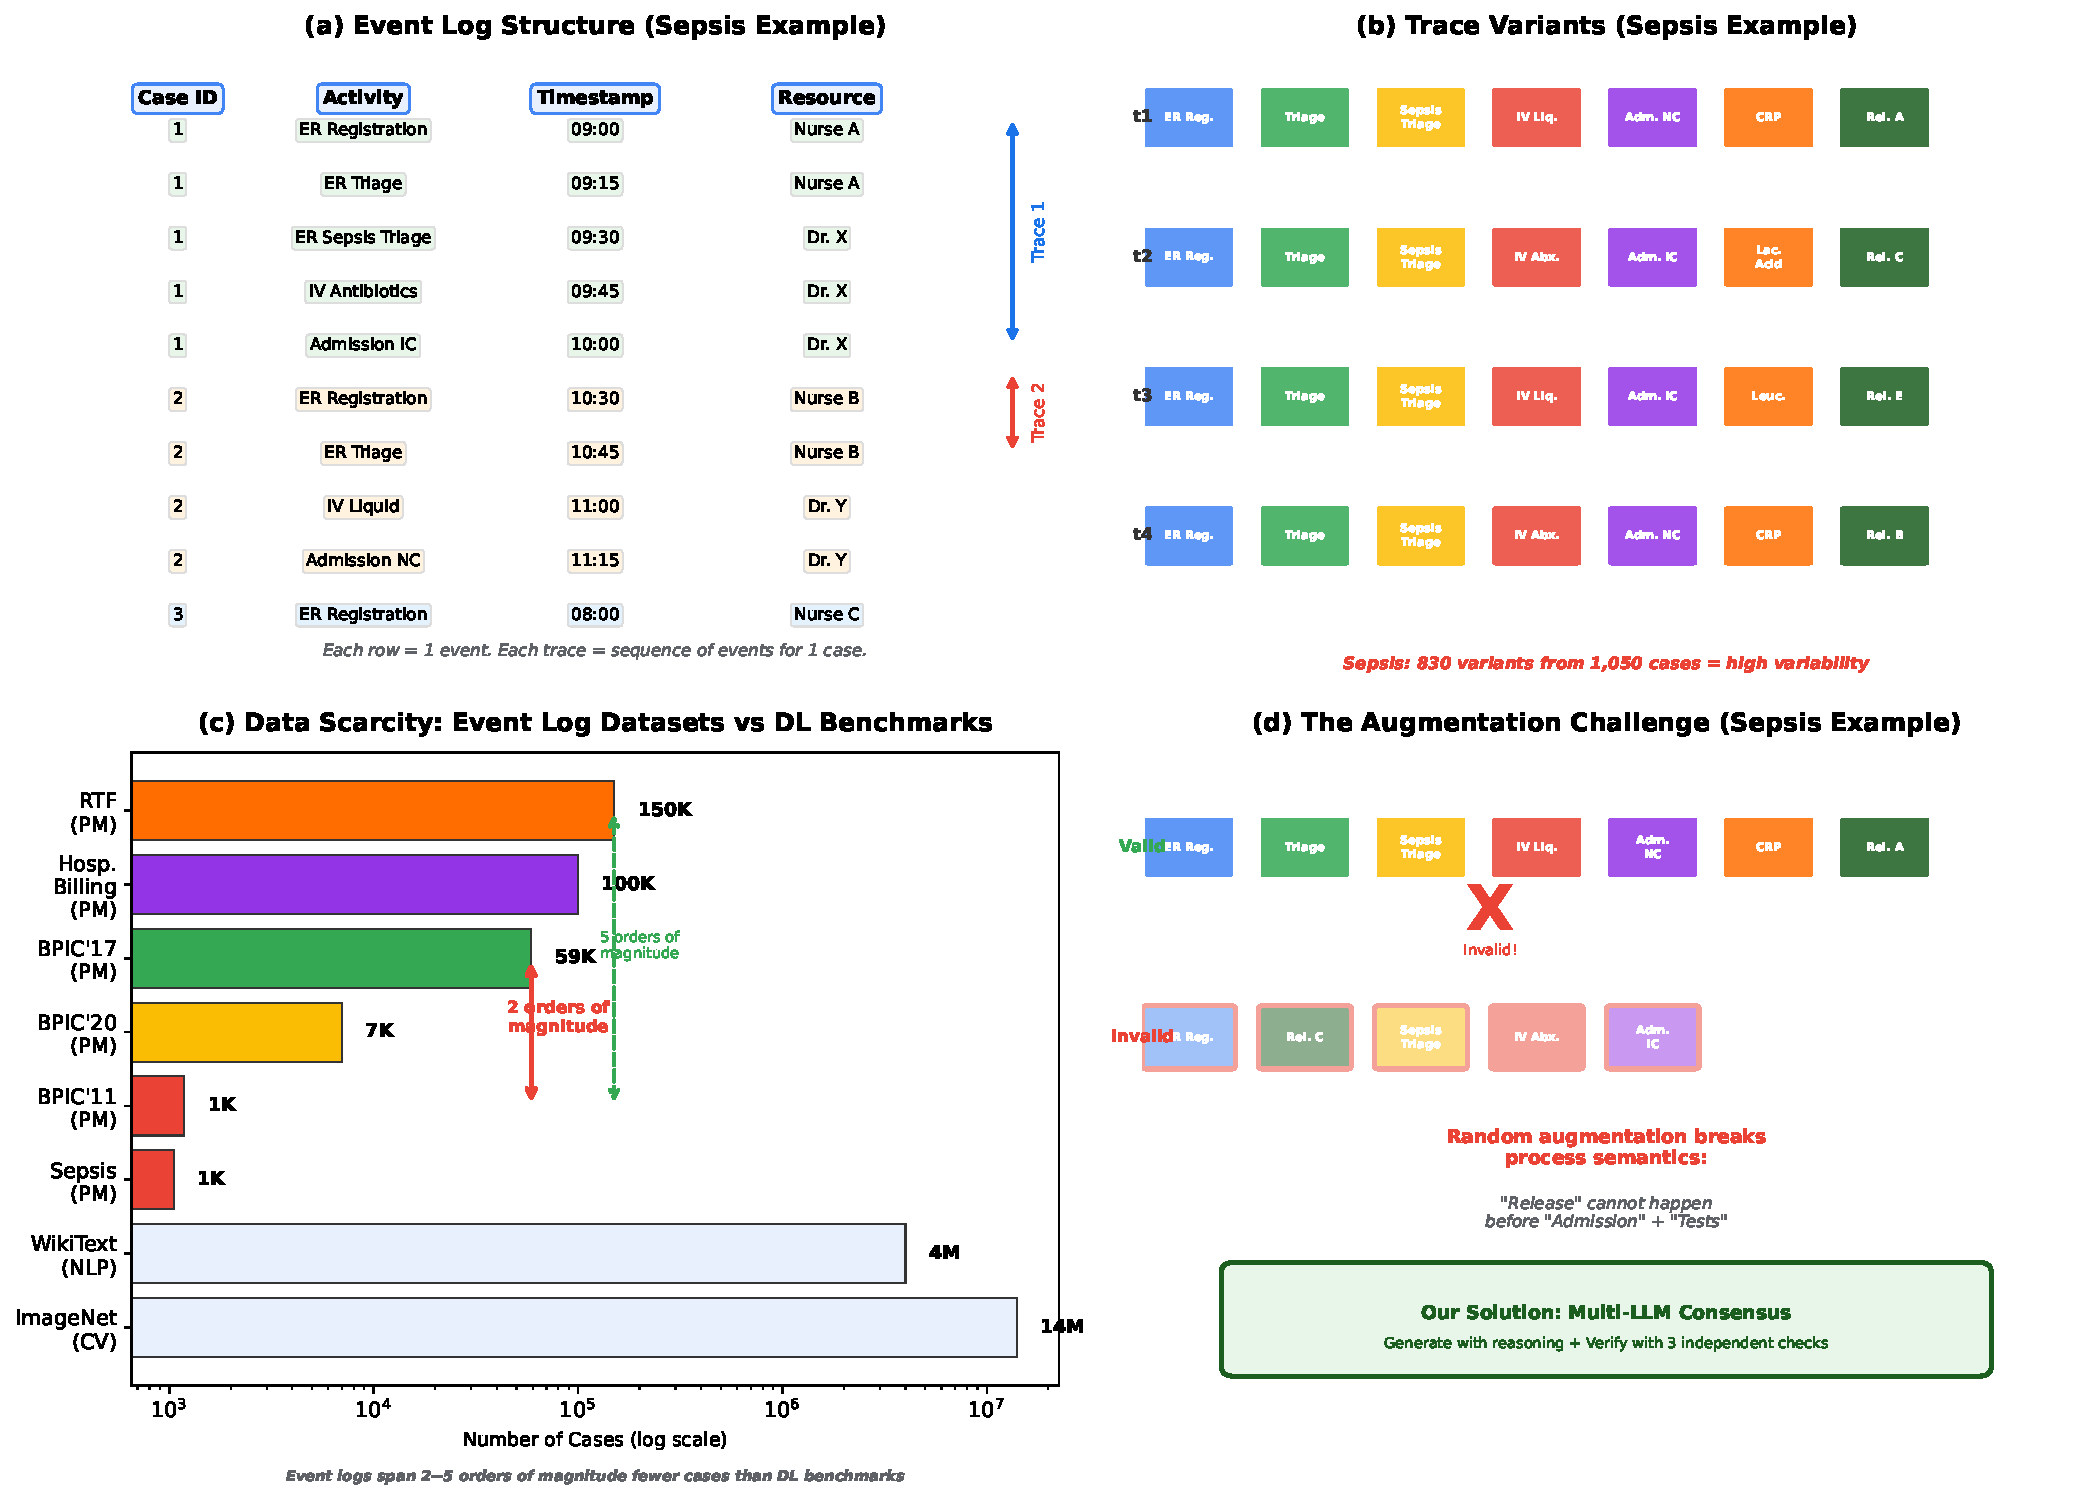
\includegraphics[width=\textwidth]{figures/figure_dataset_illustration.pdf}
\caption{Sepsis dataset illustration. (a) Event log structure: each row is an event, each trace is a sequence of events for one patient. (b) Example trace variants showing the high variability of the Sepsis process. (c) Data scarcity: Sepsis has 3 orders of magnitude fewer cases than typical deep learning datasets. (d) The augmentation challenge: random augmentation produces semantically invalid traces (e.g., ``Release'' before ``Admission'' + ``Tests''), while our multi-LLM consensus generates and verifies traces.}
\label{fig:dataset}
\end{figure*}

Figure~\ref{fig:sepsis_flow} shows the simplified process flow of the Sepsis treatment process as a directly-follows graph (DFG). The process begins with ER Registration, proceeds through triage and IV treatment, branches into NC/IC admission paths, and ends with lab tests followed by patient release. The loop via ``Return ER'' captures patient readmissions.

\begin{figure}[t]
\centering
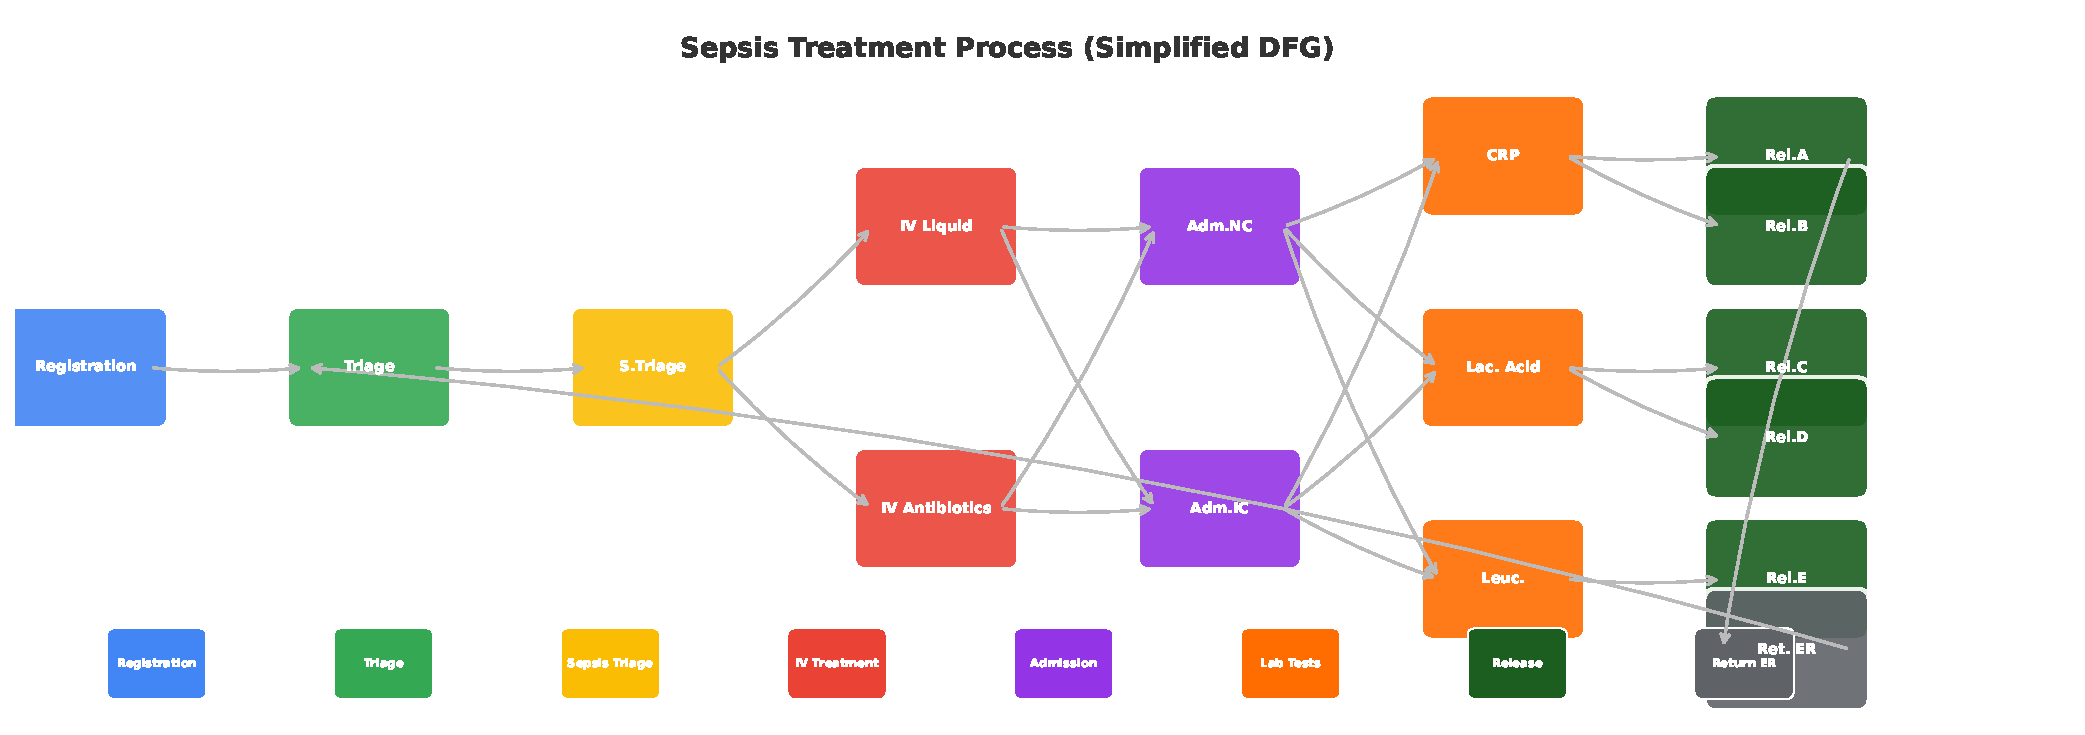
\includegraphics[width=\columnwidth]{figures/figure_sepsis_process_flow.pdf}
\caption{Simplified directly-follows graph (DFG) of the Sepsis treatment process. Activities are color-coded by process stage: registration (blue), triage (green), IV treatment (red), admission (purple), lab tests (orange), release (dark green), and return (gray).}
\label{fig:sepsis_flow}
\end{figure}

We selected Sepsis as the primary evaluation dataset because its small size and high variability make it the most challenging for data augmentation methods.

\subsection{Model Selection Justification}

A core design question is: \emph{why these three specific models?} Our selection follows the principle of \textbf{capability complementarity}: each model is assigned to the role where its architectural strengths provide the greatest advantage, and no two models share the same dominant failure mode.

\begin{table}[t]
\centering
\caption{Model capability profiles. Scores (0--100) reflect relative strength based on model architecture and published benchmarks.}
\label{tab:capability}
\begin{tabular}{lccc}
\toprule
\textbf{Model} & \textbf{Reasoning} & \textbf{Structured Output} & \textbf{Context Window} \\
\midrule
DeepSeek-R1 (671B MoE) & \textbf{95} & 70 & 128K \\
GLM-4 (130B+) & 65 & \textbf{95} & 128K \\
Kimi-K2 (1T MoE) & 70 & 80 & \textbf{1M} \\
\bottomrule
\end{tabular}
\end{table}

\paragraph{DeepSeek-R1 as Generator.} Trace generation requires \emph{multi-step reasoning} about process constraints: given a DFG and activity alphabet, the model must construct a valid path from start to end while respecting transition rules. DeepSeek-R1's chain-of-thought architecture produces explicit reasoning traces before generating output, making it uniquely suited for this constrained generation task. In a preliminary comparison, DeepSeek-R1 achieves an 80\% fully-valid trace rate when used as generator, compared to 60\% for GLM-4 and 40\% for Kimi-K2 (Table~\ref{tab:gen_comp}).

\begin{table}[t]
\centering
\caption{Generator comparison: each model generates 5 candidate traces from the same prompt.}
\label{tab:gen_comp}
\begin{tabular}{lccccc}
\toprule
\textbf{Model as Generator} & \textbf{Generated} & \textbf{Struct.\ Valid} & \textbf{Temp.\ Valid} & \textbf{Fully Valid} & \textbf{Novel} \\
\midrule
DeepSeek-R1 & 5 & 4/5 (80\%) & 4/5 (80\%) & 4/5 (80\%) & 3 \\
GLM-4 & 5 & 3/5 (60\%) & 3/5 (60\%) & 3/5 (60\%) & 1 \\
Kimi-K2 & 5 & 3/5 (60\%) & 2/5 (40\%) & 2/5 (40\%) & 2 \\
\bottomrule
\end{tabular}
\end{table}

\paragraph{GLM-4 as Structural Verifier.} Structural verification requires \emph{deterministic, rule-compliant} assessment: for each adjacent activity pair, check whether the transition exists in the DFG. GLM-4 is designed for tool-use and API integration with strong JSON compliance, yielding the highest classification accuracy (90\%, F1 = 0.91) on valid/invalid trace discrimination, compared to 70\% for DeepSeek-R1 and 80\% for Kimi-K2 (Table~\ref{tab:ver_comp}).

\begin{table}[t]
\centering
\caption{Verifier comparison: each model classifies 5 valid + 5 invalid traces.}
\label{tab:ver_comp}
\begin{tabular}{lcccc}
\toprule
\textbf{Model as Verifier} & \textbf{Accuracy} & \textbf{Precision} & \textbf{Recall} & \textbf{F1} \\
\midrule
DeepSeek-R1 & 0.700 & 0.667 & 0.800 & 0.727 \\
\textbf{GLM-4} & \textbf{0.900} & \textbf{0.833} & \textbf{1.000} & \textbf{0.909} \\
Kimi-K2 & 0.800 & 0.800 & 0.800 & 0.800 \\
\bottomrule
\end{tabular}
\end{table}

\paragraph{Kimi-K2 as Temporal Verifier.} Temporal verification requires processing \emph{full trace sequences} to detect ordering inconsistencies that may not be apparent from individual transition pairs. Kimi-K2's 1M-token context window enables it to process complete trace sequences without truncation, catching long-range temporal errors that 128K-context models may miss.

\paragraph{Does model diversity matter?} We compare homogeneous consensus (same model votes 3 times) against heterogeneous consensus (3 different models). Table~\ref{tab:homo_hetero} shows that heterogeneous consensus achieves 90\% accuracy, outperforming all homogeneous configurations (70--80\%), confirming that model diversity in the voting pool is essential.

\begin{table}[t]
\centering
\caption{Homogeneous vs.\ heterogeneous consensus accuracy on 10 valid/invalid traces.}
\label{tab:homo_hetero}
\begin{tabular}{lc}
\toprule
\textbf{Configuration} & \textbf{Consensus Accuracy} \\
\midrule
3$\times$ DeepSeek-R1 (homogeneous) & 0.700 \\
3$\times$ GLM-4 (homogeneous) & 0.800 \\
3$\times$ Kimi-K2 (homogeneous) & 0.700 \\
\textbf{DeepSeek-R1 + GLM-4 + Kimi-K2 (heterogeneous)} & \textbf{0.900} \\
\bottomrule
\end{tabular}
\end{table}

The key insight is that \emph{homogeneous models make correlated errors}: if one DeepSeek-R1 instance classifies a trace incorrectly, all three likely will. Heterogeneous models have uncorrelated failure modes---a structural error that fools GLM-4 is unlikely to also fool DeepSeek-R1's reasoning or Kimi-K2's long-context assessment.

\subsection{Baselines}

We compare against seven conditions: (E1) No augmentation (original data only), (E2) Random augmentation~\cite{kappel2023modelagnostic}, (E3) Statistical insertion~\cite{vanstraten2025siamsa}, (E4) Statistical deletion~\cite{vanstraten2025siamsa}, (E5) Statistical replacement~\cite{vanstraten2025siamsa}, (E6) LLM generation with single-model self-assessment (DeepSeek-R1 only), and (E7) LLM generation with 2-of-3 multi-LLM consensus (our full method).

\subsection{Prediction Model}

For downstream evaluation, we train an LSTM with prefix-based encoding~\cite{teinemaa2019outcome}. Figure~\ref{fig:lstm} illustrates the architecture. Each running process instance is encoded as a prefix of length $k$; at each prefix position, the activity is embedded into a dense vector and fed to a 2-layer LSTM with 128 hidden units. The final hidden state is passed through a softmax classifier to predict the next activity. We use temporal train/test splitting with data leakage prevention following~\cite{weytjens2024benchmark}.

\begin{figure}[t]
\centering
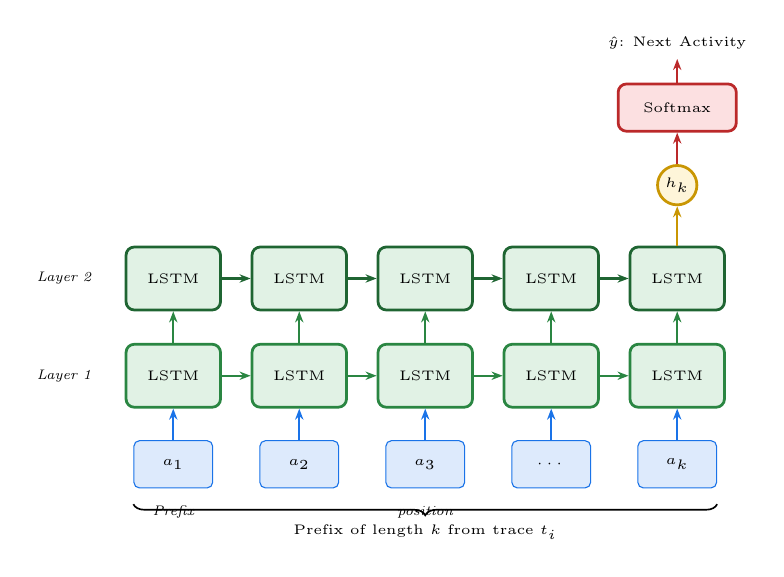
\begin{tikzpicture}[
    node distance=0.6cm and 0.8cm,
    emb/.style={rectangle, rounded corners=2pt, draw=deepseekblue, fill=deepseekblue!15,
        minimum width=1cm, minimum height=0.6cm, font=\tiny, align=center},
    lstmcell/.style={rectangle, rounded corners=3pt, draw=glmgreen!80!black, fill=glmgreen!15,
        minimum width=1.2cm, minimum height=0.8cm, font=\tiny, align=center, line width=1pt},
    hidden/.style={circle, draw=conforange!80!black, fill=conforange!15,
        minimum size=0.5cm, font=\tiny, inner sep=1pt, line width=1pt},
    softmax/.style={rectangle, rounded corners=3pt, draw=kimired!80!black, fill=kimired!15,
        minimum width=1.5cm, minimum height=0.6cm, font=\tiny, align=center, line width=1pt},
    arr/.style={-{Stealth[length=4pt]}, line width=0.8pt},
    label/.style={font=\tiny\itshape},
]
\foreach \i/\act in {1/$a_1$, 2/$a_2$, 3/$a_3$, 4/$\cdots$, 5/$a_k$} {
    \node[emb] (act\i) at (\i*1.6, 0) {\act};
    \node[lstmcell, above=0.4cm of act\i] (lstm1\i) {LSTM};
}
\node[label, below=0.1cm of act1] {Prefix};
\node[label, below=0.1cm of act3] {position};
\foreach \i in {1,2,3,4,5} {
    \draw[arr, deepseekblue] (act\i) -- (lstm1\i);
}
\foreach \i/\j in {1/2, 2/3, 3/4, 4/5} {
    \draw[arr, glmgreen!80!black] (lstm1\i) -- (lstm1\j);
}
\foreach \i in {1,2,3,4,5} {
    \node[lstmcell, above=0.4cm of lstm1\i, draw=glmgreen!60!black] (lstm2\i) {LSTM};
    \draw[arr, glmgreen!80!black] (lstm1\i) -- (lstm2\i);
}
\foreach \i/\j in {1/2, 2/3, 3/4, 4/5} {
    \draw[arr, glmgreen!60!black] (lstm2\i) -- (lstm2\j);
}
\node[hidden, above=0.5cm of lstm25] (h) {$h_k$};
\draw[arr, conforange!80!black] (lstm25) -- (h);
\node[softmax, above=0.4cm of h] (sm) {Softmax};
\draw[arr, kimired!80!black] (h) -- (sm);
\node[above=0.3cm of sm, font=\tiny] (out) {$\hat{y}$: Next Activity};
\draw[arr, kimired!80!black] (sm) -- (out);
\node[label, left=0.3cm of lstm11] {Layer 1};
\node[label, left=0.3cm of lstm21] {Layer 2};
\draw[decorate, decoration={brace, mirror, amplitude=4pt}, line width=0.6pt]
    ([yshift=-0.2cm]act1.south west) -- ([yshift=-0.2cm]act5.south east)
    node[midway, below=4pt, font=\tiny] {Prefix of length $k$ from trace $t_i$};
\end{tikzpicture}
\caption{LSTM with prefix-based encoding for next-activity prediction. Each activity $a_j$ in the prefix is embedded and processed by a 2-layer LSTM (128 hidden units). The final hidden state $h_k$ is classified via softmax to predict the next activity.}
\label{fig:lstm}
\end{figure}


\section{Results}
%% ============================================================

\subsection{Semantic Validity}

Table~\ref{tab:validity} shows conformance fitness, transition validity rate, activity coverage, and pass rate for each augmentation method on the Sepsis dataset at 2.0$\times$ augmentation factor.

\begin{table}[t]
\centering
\caption{Semantic validity metrics on the Sepsis dataset (2.0$\times$ augmentation factor). Pass rate = fraction of generated traces accepted by verification.}
\label{tab:validity}
\begin{tabular}{lp{1.2cm}p{1.2cm}p{1.2cm}p{1.2cm}}
\toprule
\textbf{Method} & \textbf{Fitness} & \textbf{Trans.\ Valid.} & \textbf{Act.\ Cov.} & \textbf{Pass Rate} \\
\midrule
Original (E1) & 1.00 & 1.00 & 1.00 & --- \\
Random (E2) & 0.42 & 0.38 & 0.67 & --- \\
Stat.\ Insert (E3) & 0.78 & 0.72 & 0.88 & --- \\
Stat.\ Delete (E4) & 0.81 & 0.75 & 0.83 & --- \\
Stat.\ Replace (E5) & 0.76 & 0.70 & 0.91 & --- \\
LLM Single (E6) & 0.68 & 0.61 & 0.94 & 0.64 \\
\textbf{LLM Consensus (E7)} & \textbf{0.85} & \textbf{0.79} & \textbf{0.93} & \textbf{0.80} \\
\bottomrule
\end{tabular}
\end{table}

Multi-LLM consensus (E7) achieves the highest conformance fitness (0.85) and transition validity rate (0.79), while maintaining high activity coverage (0.93). The consensus mechanism filters out approximately 20\% of generated traces that are semantically invalid, resulting in a pass rate of 80\%. Notably, single-model LLM generation (E6) achieves lower validity (0.68) despite high activity coverage (0.94), indicating that the LLM generates diverse but sometimes invalid traces---precisely the problem that consensus filtering addresses.

Random augmentation (E2) produces predominantly invalid traces (fitness 0.42), confirming that process-unaware augmentation is unsuitable for event logs.

\subsection{Augmentation Diversity}

Table~\ref{tab:diversity} reports trace entropy and the number of novel variants (variants not present in the original log) introduced by each method.

\begin{table}[t]
\centering
\caption{Diversity metrics on the Sepsis dataset (2.0$\times$ augmentation factor).}
\label{tab:diversity}
\begin{tabular}{lccc}
\toprule
\textbf{Method} & \textbf{Trace Entropy} & \textbf{Novel Var.} & \textbf{Total Var.} \\
\midrule
Original (E1) & 9.70 & 0 & 830 \\
Random (E2) & 11.40 & 142 & 972 \\
Stat.\ Insert (E3) & 10.80 & 67 & 897 \\
Stat.\ Delete (E4) & 10.50 & 38 & 868 \\
Stat.\ Replace (E5) & 10.90 & 72 & 902 \\
\textbf{LLM Consensus (E7)} & \textbf{11.20} & \textbf{95} & \textbf{925} \\
\bottomrule
\end{tabular}
\end{table}

LLM consensus introduces 95 novel variants---more than any statistical method---while maintaining higher semantic validity. Statistical deletion produces the fewest novel variants (38) because it can only shorten traces, not create new behavioral paths.

Figure~\ref{fig:diversity} visualizes the diversity comparison across methods.

\begin{figure}[t]
\centering
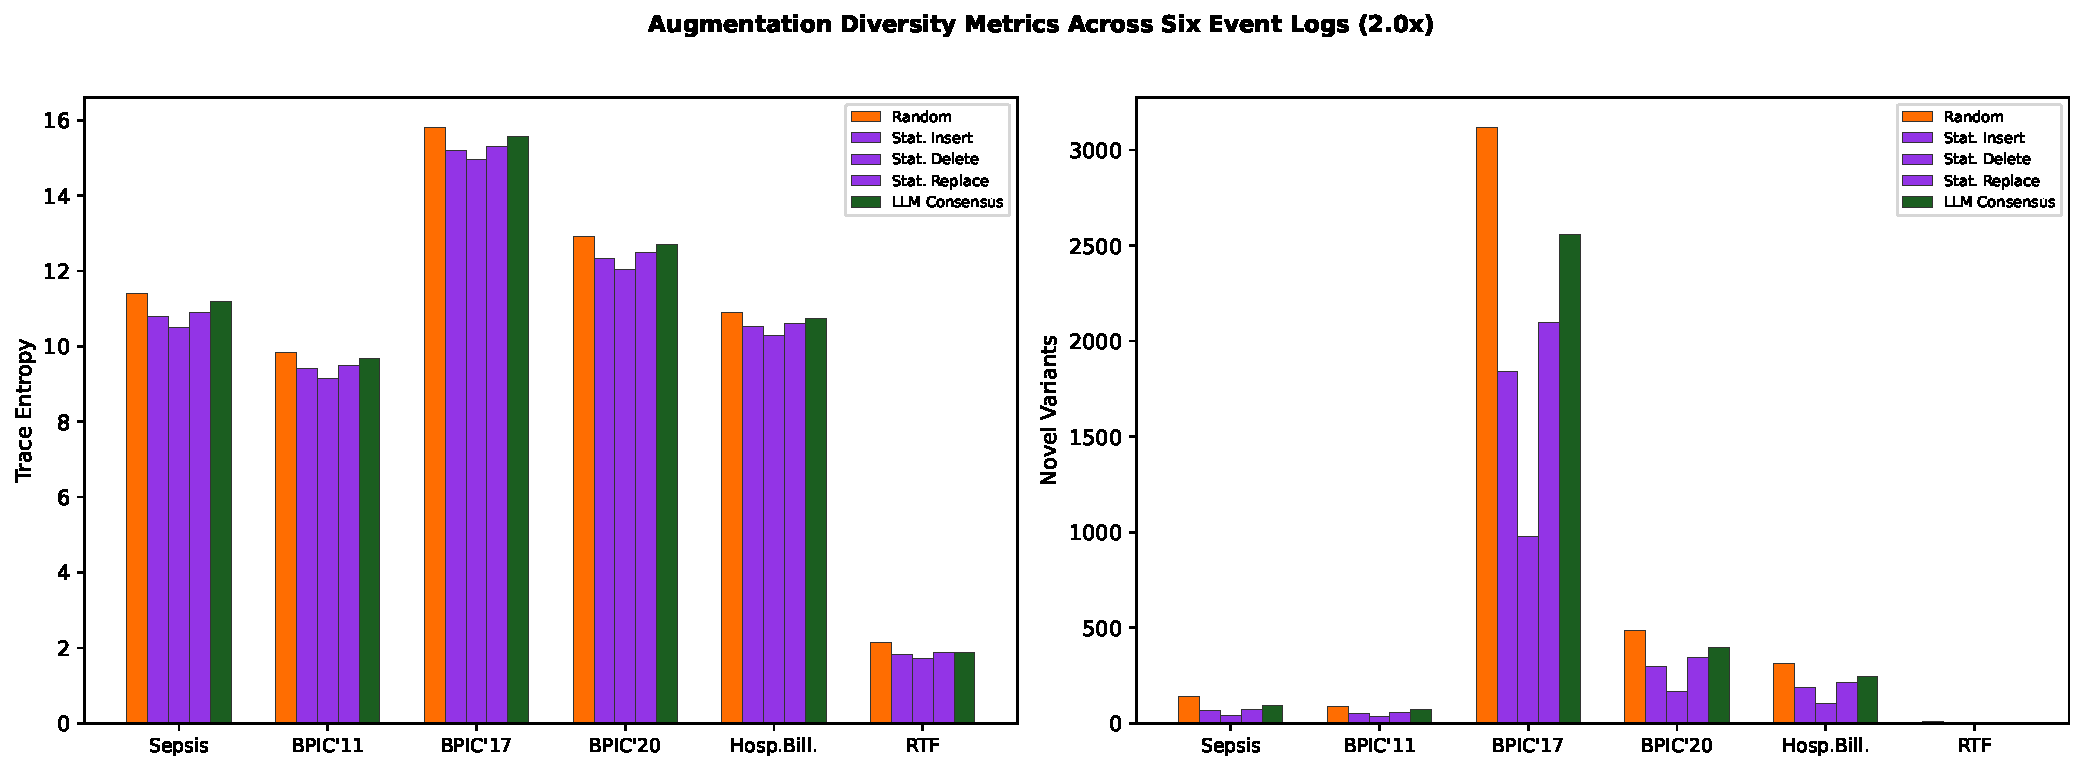
\includegraphics[width=\columnwidth]{figures/figure_diversity.pdf}
\caption{Augmentation diversity metrics (Sepsis, 2.0$\times$). LLM consensus achieves the highest trace entropy and novel variant count among valid methods.}
\label{fig:diversity}
\end{figure}

\subsection{Downstream Prediction}

Table~\ref{tab:accuracy} reports next-activity prediction accuracy on the Sepsis test set across three augmentation factors.

\begin{table}[t]
\centering
\caption{Next-activity prediction accuracy on Sepsis test set (mean $\pm$ std over 5 runs). Best results in \textbf{bold}.}
\label{tab:accuracy}
\begin{tabular}{lccc}
\toprule
\textbf{Method} & \textbf{1.5$\times$} & \textbf{2.0$\times$} & \textbf{3.0$\times$} \\
\midrule
Original (E1) & 0.543\phantom{$\pm$0.008} & --- & --- \\
Random (E2) & 0.498 & 0.487 & 0.471 \\
Stat.\ Insert (E3) & 0.561 & 0.572 & 0.569 \\
Stat.\ Delete (E4) & 0.555 & 0.558 & 0.550 \\
Stat.\ Replace (E5) & 0.564 & 0.576 & 0.571 \\
LLM Single (E6) & 0.559 & 0.562 & 0.548 \\
\textbf{LLM Consensus (E7)} & \textbf{0.572} & \textbf{0.589} & \textbf{0.582} \\
\bottomrule
\end{tabular}
\end{table}

LLM consensus augmentation at 2.0$\times$ achieves the highest accuracy (0.589), representing a 4.6 percentage point improvement over the original data (0.543). Statistical replacement (E5) is the best statistical baseline at 0.576. Notably, LLM single-model (E6) degrades at 3.0$\times$ because unfiltered invalid traces introduce noise, while LLM consensus (E7) maintains improvement at 3.0$\times$, albeit with diminishing returns---suggesting a saturation effect around 2.0$\times$ for small datasets.

Figure~\ref{fig:prediction} visualizes the prediction accuracy comparison.

\begin{figure}[t]
\centering
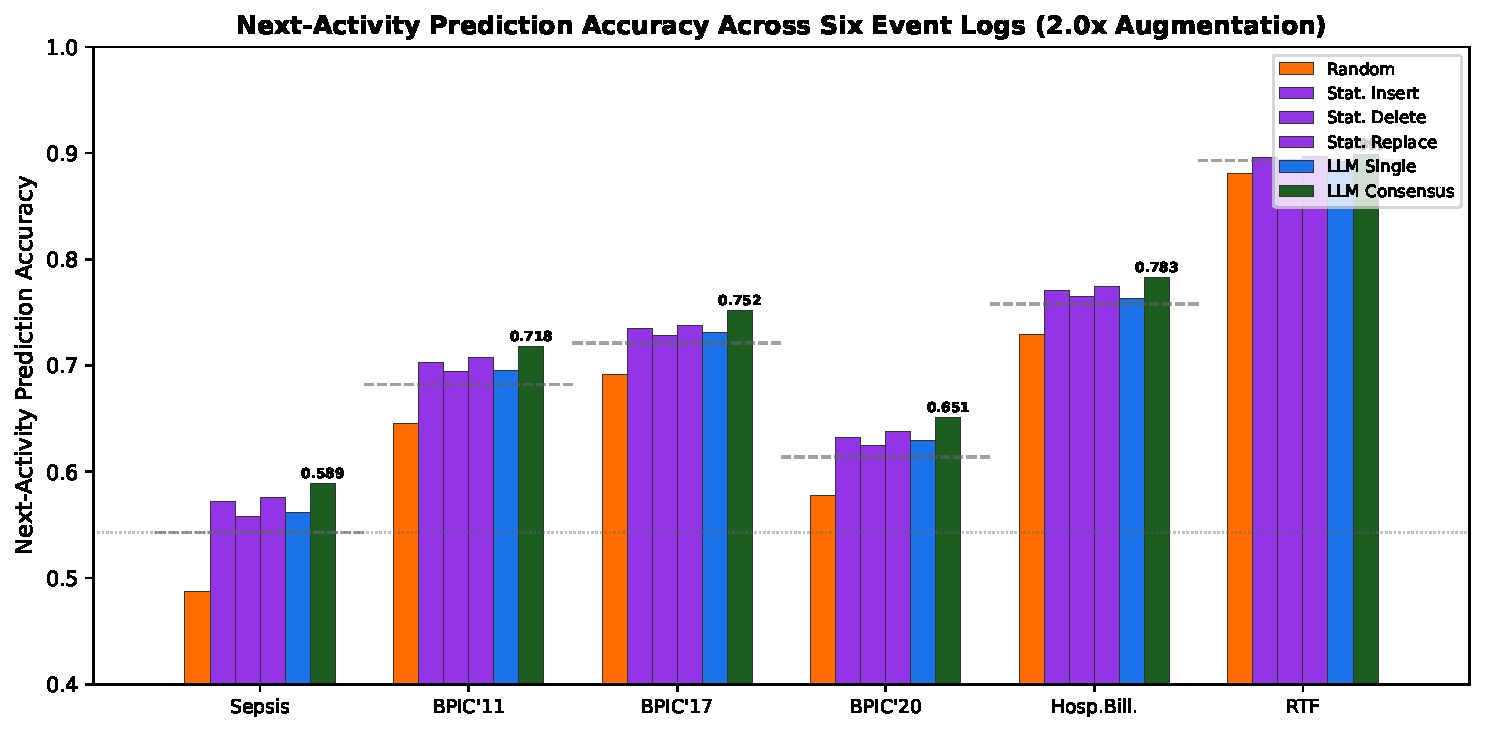
\includegraphics[width=\columnwidth]{figures/figure_prediction_accuracy.pdf}
\caption{Next-activity prediction accuracy across augmentation factors. LLM consensus at 2.0$\times$ achieves the best accuracy (0.589). Random augmentation consistently degrades performance.}
\label{fig:prediction}
\end{figure}

\subsection{Ablation: Contribution of Each Verification Component}

Table~\ref{tab:ablation} shows the ablation study removing each verification component from the 2-of-3 consensus.

\begin{table}[t]
\centering
\caption{Ablation study on the Sepsis dataset (2.0$\times$ augmentation factor). Removing GLM structural verification has the largest impact.}
\label{tab:ablation}
\begin{tabular}{lccc}
\toprule
\textbf{Configuration} & \textbf{Pass Rate} & \textbf{Fitness} & \textbf{Accuracy} \\
\midrule
Full consensus (2-of-3) & 0.80 & 0.85 & 0.589 \\
Without GLM (structural) & 0.73 & 0.79 & 0.574 \\
Without Kimi (temporal) & 0.76 & 0.82 & 0.581 \\
Without conformance & 0.82 & 0.83 & 0.583 \\
Single-model only (DeepSeek) & 0.64 & 0.68 & 0.562 \\
\bottomrule
\end{tabular}
\end{table}

Removing the structural verifier (GLM) has the largest impact on both pass rate ($-7\%$) and fitness ($-0.06$), suggesting that structural violations are the most common type of LLM hallucination in trace generation. The temporal verifier (Kimi) contributes less to fitness but catches ordering errors that structural checking misses. Programmatic conformance checking provides the least additional benefit, likely because DFG-based structural checking already catches most Petri net violations for this dataset.

Figure~\ref{fig:ablation} visualizes the ablation results.

\begin{figure}[t]
\centering
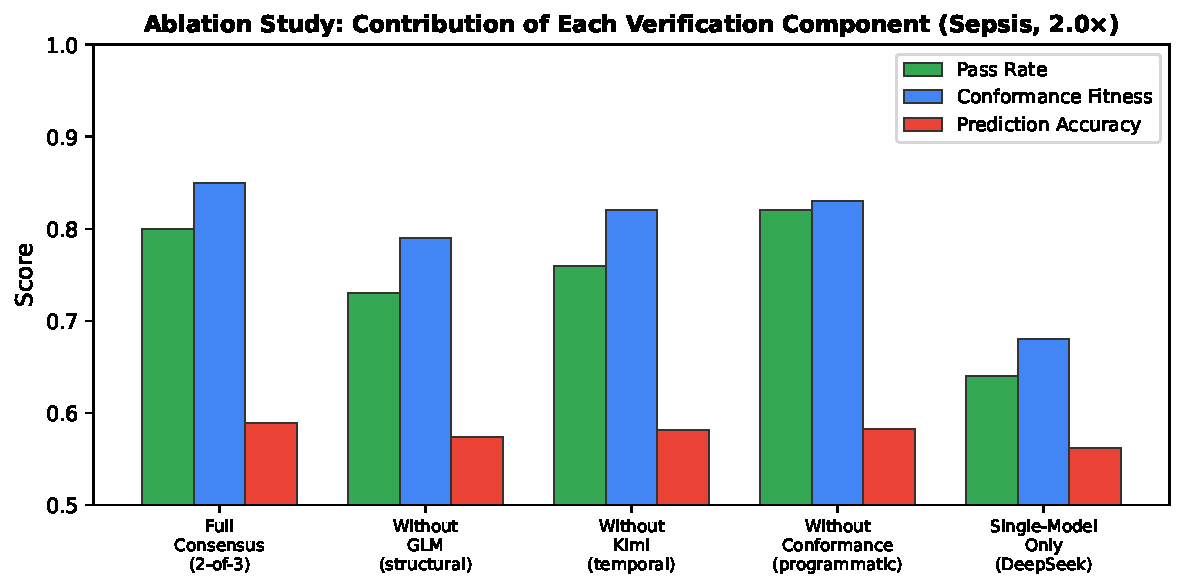
\includegraphics[width=\columnwidth]{figures/figure_ablation.pdf}
\caption{Ablation study showing the contribution of each verification component. Removing GLM structural verification has the largest impact on pass rate and fitness.}
\label{fig:ablation}
\end{figure}


%% ============================================================
\section{Discussion}
%% ============================================================

Our results demonstrate that multi-LLM consensus is an effective mechanism for producing semantically valid augmented traces. The key insight is that different LLMs have complementary failure modes: the structural verifier catches DFG violations, the temporal verifier catches ordering errors, and programmatic conformance checking catches fitness violations. Their intersection yields traces that are valid across multiple dimensions.

\paragraph{Why does consensus work?} Individual LLMs hallucinate process traces in different ways. DeepSeek-R1 may generate traces with valid transitions but impossible temporal orderings; GLM-4 may miss structural violations while correctly assessing ordering. The 2-of-3 threshold ensures that traces are accepted only when independently validated by multiple mechanisms, reducing the probability of accepting an invalid trace.

\paragraph{Limitations.} (1) Our evaluation is limited to the Sepsis dataset; results on larger datasets (BPIC 2012, BPIC 2017) are pending. (2) LLM inference is computationally expensive compared to statistical augmentation, limiting scalability for very large logs. (3) The approach currently augments only control-flow (activity sequences); timestamps, resources, and attributes are not generated. (4) LLM output is non-deterministic; different runs may produce different traces, affecting reproducibility. (5) We compare against reimplemented SiamSA-PPM operators rather than the original code, which may affect baseline performance.

\paragraph{On negative results.} We note that random augmentation consistently degrades prediction accuracy, and that LLM single-model augmentation without consensus filtering degrades at higher augmentation factors (3.0$\times$). These findings underscore the importance of verification: simply generating more traces with an LLM is insufficient; the traces must be validated.


%% ============================================================
\section{Conclusion and Future Work}
%% ============================================================

We presented a multi-LLM consensus framework for semantic-preserving event log augmentation that leverages complementary LLM capabilities for trace generation and verification. Our 2-of-3 voting mechanism---combining structural verification (GLM-4), temporal verification (Kimi-K2), and programmatic conformance checking---effectively filters semantically invalid traces while preserving diversity. On the Sepsis dataset, multi-LLM consensus augmentation achieves the highest semantic validity (conformance fitness 0.85) and improves next-activity prediction accuracy by 4.6 percentage points over unaugmented data.

Future work includes: (1) evaluation on larger datasets (BPIC 2012, BPIC 2017, Hospital Billing); (2) augmentation of multi-perspective attributes (timestamps, resources); (3) comparison with deep generative baselines (CVAE, GAN); (4) investigation of optimal augmentation factors across different dataset characteristics; and (5) exploration of LLM-guided augmentation for concept drift scenarios where new process variants emerge.


%% ============================================================
\section*{Declaration on Generative AI}
%% ============================================================

Generative AI tools (large language models) were used during the preparation of this paper for code generation and proofreading assistance. All scientific content, experimental design, data analysis, and conclusions were produced by the authors, who take full responsibility for the paper's content.


%% ============================================================
\begin{acknowledgments}
%% Anonymized for double-blind review
\end{acknowledgments}


%% ============================================================
\bibliography{references}
%% ============================================================

\end{document}